\begin{frame}
\frametitle{Civil Aviation in Australia}
\begin{itemize}
\item<1-> Federally regulated by Civil Aviation Safety Authority (CASA).
\item<2-> Services, such as weather reporting, provided by Airservices
          Australia.
\end{itemize}
\end{frame}

\begin{frame}
\frametitle{Civil Aviation in Australia}
\begin{block}{and we don't want this to happen}
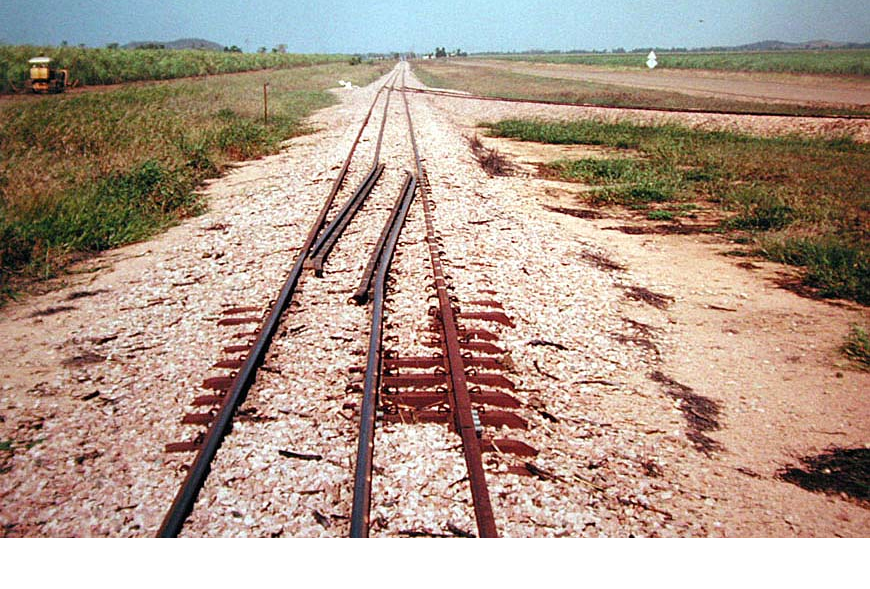
\includegraphics[height=0.5\textheight]{image/railway-gauge.png}
\end{block}
\begin{block}{}
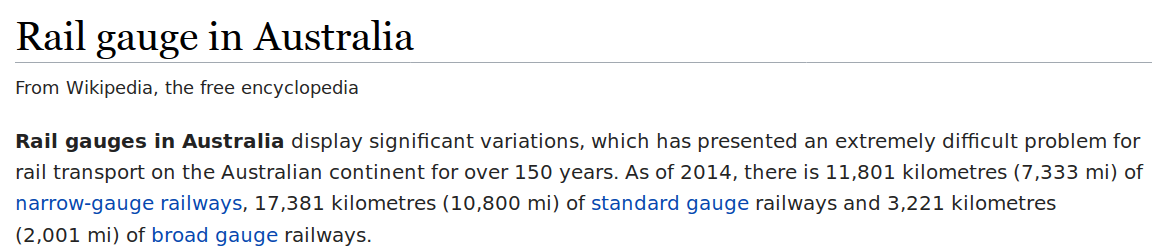
\includegraphics[height=0.2\textheight]{image/railway-gauge-wikipedia.png}
\end{block}
\end{frame}

\begin{frame}
\frametitle{Civil Aviation internationally}
\begin{block}{so these also exist}
\begin{itemize}
\item<1-> International Air Services Commission (IASC).
\item<2-> International Civil Aviation Organisation (ICAO).
\end{itemize}
\end{block}
\end{frame}

\begin{frame}
\frametitle{Civil Aviation internationally}
\begin{block}{India}
\begin{itemize}
\item<1-> India is one of 191 ICAO member states.
\item<1-> India is one of 36 ICAO elected governing councils.
\item<2-> Like Australia!
\end{itemize}
\end{block}
\end{frame}

\begin{frame}
\frametitle{Civil Aviation in Australia}
\begin{block}{Australian aviation legislation}
\begin{itemize}
\item<1-> Civil Aviation Act 1988 (CAA1988).
\item<2-> Under CAA1988, is Civil Aviation Safety Regulations 1998 (CASR1998).
\item<3-> There are also Civil Aviation Orders (CAO).
\item<4-> and Civil Aviation Advisory Publications (CAAP).
\end{itemize}
\end{block}
\end{frame}
